%*******************************************************************************
% * Copyright (c) 2006-2013 
% * Institute of Automation, Dresden University of Technology
% * 
% * All rights reserved. This program and the accompanying materials
% * are made available under the terms of the Eclipse Public License v1.0 
% * which accompanies this distribution, and is available at
% * http://www.eclipse.org/legal/epl-v10.html
% * 
% * Contributors:
% *   Institute of Automation - TU Dresden, Germany 
% *      - initial API and implementation
% ******************************************************************************/

%%%%%%%%%%%%%%%%%%%%%%%%%%%%%%%%%%%%%%%%%%%%%%%%%%%%%%%%%%%%%%%%%%%%%%
%%%%%%%%%%%%%%%%%%%%%%%%%%%%%%%%%%%%%%%%%%%%%%%%%%%%%%%%%%%%%%%%%%%%%%  
\chapter{Sonstiges}
\label{sec:Sonstiges}

%%%%%%%%%%%%%%%%%%%%%%%%%%%%%%%%%%%%%%%%%%%%%%%%%%%%%%%%%%%%%%%%%%%%%%
\section{Postergestaltung}
\label{sec:Postergestaltung}
%%%%%%%%%%%%%%%%%%%%%%%%%%%%%%%%%%%%%%%%%%%%%%%%%%%%%%%%%%%%%%%%%%%%%%

(Beispiele siehe Postertafel des Instituts)

\minisec{Vorlage}
Eine \LaTeX{}-Vorlage für das Poster kann auf der \href{http://www.et.tu-dresden.de/ifa/index.php?id=330}{Internetseite des Instituts} heruntergeladen werden.

\minisec{Schwerpunkte}
\begin{compactitem}
  \item Kurzvorstellung der Aufgabe
  \item Anschauliche Darstellung des Lösungsweges und wesentlicher Ergebnisse, möglichst durch Bilder und Tabellen unterstützt (kurze Texte, 14 pt / 3mm)
  \item Zusammenfassende Wertung der Ergebnisse und Ausblick auf noch zu lösende Probleme.
\end{compactitem}

\minisec{Gestaltung}
\begin{compactitem}
  \item Größe: 
    \begin{compactitem}
      \item DIN A2-Querformat (59,4 x 42,0 cm), allseitiger Rand 2 cm
  \end{compactitem}
  \item Kopf:
    \begin{compactitem}
      \item Überschrift (Kurzthema), Schriftgröße: 90 pt, fett (20 mm)
      \item Logo-Block (Schriftgröße: 18 pt (4 mm) / 14 pt (3 mm):
    \end{compactitem}
\end{compactitem}

\begin{figure}[ht]
  \centering
  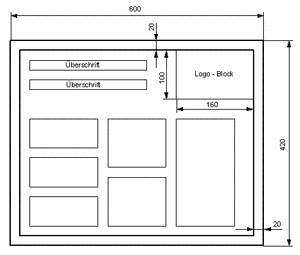
\includegraphics[keepaspectratio, width=9cm]{example_files/RTEmagicC_poster.jpg}
  \caption{Gestaltungsrichtlinie des Posters, Maße und Abstände}
  \label{fig:poster}
\end{figure}

\minisec{Gestaltung des Logo-Blocks}
Maße und Schriftgrößen siehe oben und in Abbildungen \ref{fig:poster} und \ref{fig:poster-logo-block}

\begin{figure}[ht]
  \centering
  
\includegraphics[keepaspectratio, width=9cm]{example_files/RTEmagicC_muster.jpg}
  \caption{Gestaltungsrichtlinie des Logo-Blocks des Posters}
  \label{fig:poster-logo-block}
\end{figure}


%%%%%%%%%%%%%%%%%%%%%%%%%%%%%%%%%%%%%%%%%%%%%%%%%%%%%%%%%%%%%%%%%%%%%%
\section{Informationsmittel zur Literaturrecherche}
\label{sec:InformationsmittelZurLiteraturrecherche}
%%%%%%%%%%%%%%%%%%%%%%%%%%%%%%%%%%%%%%%%%%%%%%%%%%%%%%%%%%%%%%%%%%%%%%

Wegen der ständig anwachsenden Zahl von Veröffentlichungen ist es angebracht, bei der Literaturrecherche rationelle Methoden anzuwenden.
Dafür stehen in den wissenschaftlichen Bibliotheken
\begin{compactitem}
  \item Sächsische Landesbibliothek -- Staats- und Universitätsbibliothek (SLUB)
  \item Fachbibliothek Elektrotechnik und Informationstechnik (FBE, DrePunct, Zellescher Weg 17)
\end{compactitem}
Informationsmittel zur Verfügung.

\begin{table*}[h]
  \centering
  \caption{Kataloge}
  \label{tab:Kataloge}
  \begin{tabular}{lll}%{p{4cm}p{4cm}p{4cm}}
    \toprule
    Bezeichnung     &                                                   & Standort  \\
    \midrule
    {\bfseries Kataloge}  & Alphabetischer Katalog                      & SLUB, FBE \\
                    & Sachkatalog                                       & SLUB, FBE \\
                    & Dissertationskatalog                              & SLUB, FBE \\
                    & Zeitschriftenkatalog                              & SLUB, FBE \\
                    & Zentralkatalog                                    & SLUB      \\
    \multicolumn{2}{l}{Bibliographien}                                  & SLUB, FBE \\
    \multicolumn{2}{l}{Firmenschriften/Prospekte/Wirtschaftsliteratur}  & SLUB      \\
    \multicolumn{2}{l}{Normen}                                          & SLUB, FBE \\
    \multicolumn{2}{l}{Dokumentations- und Referatedienste}             & SLUB, FBE \\
    \multicolumn{2}{l}{Patente}                                         & SLUB\\
    \bottomrule
  \end{tabular}
\end{table*}

\minisec{Rechnergestützte Recherche-Mittel}
\begin{compactitem}
  \item Rechnergestützter Katalog OPAC (Monographie-Bestand der SLUB)
  \item Recherchen in CD-ROM-Datenbanken verschiedener Hersteller (SLUB)
  \item IEEE-Dokumente: Aufsätze, Tagungsbandbeiträge etc. (Volltexte seit 1951 von Uni-IP)
  \item TOC Premier: Zeitschrifteninhaltsverzeichnisse führender Verlage weltweit (Literaturrecherche von Uni-IP)
  \item Datenbank FIZ Technik und Unterdatenbanken: (Literaturrecherche von Uni-IP)
  \item Online-Informationsdienst in kostenpflichtigen Datenbanken (SLUB)
  \item Internet
\end{compactitem}